\documentclass[]{article}
\usepackage{lmodern}
\usepackage{amssymb,amsmath}
\usepackage{ifxetex,ifluatex}
\usepackage{fixltx2e} % provides \textsubscript
\ifnum 0\ifxetex 1\fi\ifluatex 1\fi=0 % if pdftex
  \usepackage[T1]{fontenc}
  \usepackage[utf8]{inputenc}
\else % if luatex or xelatex
  \ifxetex
    \usepackage{mathspec}
  \else
    \usepackage{fontspec}
  \fi
  \defaultfontfeatures{Ligatures=TeX,Scale=MatchLowercase}
\fi
% use upquote if available, for straight quotes in verbatim environments
\IfFileExists{upquote.sty}{\usepackage{upquote}}{}
% use microtype if available
\IfFileExists{microtype.sty}{%
\usepackage{microtype}
\UseMicrotypeSet[protrusion]{basicmath} % disable protrusion for tt fonts
}{}
\usepackage[margin=1in]{geometry}
\usepackage{hyperref}
\hypersetup{unicode=true,
            pdftitle={An Introduction to Dixon-Coles Modelling in R (part 1)},
            pdfauthor={Robert Hickman},
            pdfborder={0 0 0},
            breaklinks=true}
\urlstyle{same}  % don't use monospace font for urls
\usepackage{color}
\usepackage{fancyvrb}
\newcommand{\VerbBar}{|}
\newcommand{\VERB}{\Verb[commandchars=\\\{\}]}
\DefineVerbatimEnvironment{Highlighting}{Verbatim}{commandchars=\\\{\}}
% Add ',fontsize=\small' for more characters per line
\usepackage{framed}
\definecolor{shadecolor}{RGB}{248,248,248}
\newenvironment{Shaded}{\begin{snugshade}}{\end{snugshade}}
\newcommand{\KeywordTok}[1]{\textcolor[rgb]{0.13,0.29,0.53}{\textbf{#1}}}
\newcommand{\DataTypeTok}[1]{\textcolor[rgb]{0.13,0.29,0.53}{#1}}
\newcommand{\DecValTok}[1]{\textcolor[rgb]{0.00,0.00,0.81}{#1}}
\newcommand{\BaseNTok}[1]{\textcolor[rgb]{0.00,0.00,0.81}{#1}}
\newcommand{\FloatTok}[1]{\textcolor[rgb]{0.00,0.00,0.81}{#1}}
\newcommand{\ConstantTok}[1]{\textcolor[rgb]{0.00,0.00,0.00}{#1}}
\newcommand{\CharTok}[1]{\textcolor[rgb]{0.31,0.60,0.02}{#1}}
\newcommand{\SpecialCharTok}[1]{\textcolor[rgb]{0.00,0.00,0.00}{#1}}
\newcommand{\StringTok}[1]{\textcolor[rgb]{0.31,0.60,0.02}{#1}}
\newcommand{\VerbatimStringTok}[1]{\textcolor[rgb]{0.31,0.60,0.02}{#1}}
\newcommand{\SpecialStringTok}[1]{\textcolor[rgb]{0.31,0.60,0.02}{#1}}
\newcommand{\ImportTok}[1]{#1}
\newcommand{\CommentTok}[1]{\textcolor[rgb]{0.56,0.35,0.01}{\textit{#1}}}
\newcommand{\DocumentationTok}[1]{\textcolor[rgb]{0.56,0.35,0.01}{\textbf{\textit{#1}}}}
\newcommand{\AnnotationTok}[1]{\textcolor[rgb]{0.56,0.35,0.01}{\textbf{\textit{#1}}}}
\newcommand{\CommentVarTok}[1]{\textcolor[rgb]{0.56,0.35,0.01}{\textbf{\textit{#1}}}}
\newcommand{\OtherTok}[1]{\textcolor[rgb]{0.56,0.35,0.01}{#1}}
\newcommand{\FunctionTok}[1]{\textcolor[rgb]{0.00,0.00,0.00}{#1}}
\newcommand{\VariableTok}[1]{\textcolor[rgb]{0.00,0.00,0.00}{#1}}
\newcommand{\ControlFlowTok}[1]{\textcolor[rgb]{0.13,0.29,0.53}{\textbf{#1}}}
\newcommand{\OperatorTok}[1]{\textcolor[rgb]{0.81,0.36,0.00}{\textbf{#1}}}
\newcommand{\BuiltInTok}[1]{#1}
\newcommand{\ExtensionTok}[1]{#1}
\newcommand{\PreprocessorTok}[1]{\textcolor[rgb]{0.56,0.35,0.01}{\textit{#1}}}
\newcommand{\AttributeTok}[1]{\textcolor[rgb]{0.77,0.63,0.00}{#1}}
\newcommand{\RegionMarkerTok}[1]{#1}
\newcommand{\InformationTok}[1]{\textcolor[rgb]{0.56,0.35,0.01}{\textbf{\textit{#1}}}}
\newcommand{\WarningTok}[1]{\textcolor[rgb]{0.56,0.35,0.01}{\textbf{\textit{#1}}}}
\newcommand{\AlertTok}[1]{\textcolor[rgb]{0.94,0.16,0.16}{#1}}
\newcommand{\ErrorTok}[1]{\textcolor[rgb]{0.64,0.00,0.00}{\textbf{#1}}}
\newcommand{\NormalTok}[1]{#1}
\usepackage{graphicx,grffile}
\makeatletter
\def\maxwidth{\ifdim\Gin@nat@width>\linewidth\linewidth\else\Gin@nat@width\fi}
\def\maxheight{\ifdim\Gin@nat@height>\textheight\textheight\else\Gin@nat@height\fi}
\makeatother
% Scale images if necessary, so that they will not overflow the page
% margins by default, and it is still possible to overwrite the defaults
% using explicit options in \includegraphics[width, height, ...]{}
\setkeys{Gin}{width=\maxwidth,height=\maxheight,keepaspectratio}
\IfFileExists{parskip.sty}{%
\usepackage{parskip}
}{% else
\setlength{\parindent}{0pt}
\setlength{\parskip}{6pt plus 2pt minus 1pt}
}
\setlength{\emergencystretch}{3em}  % prevent overfull lines
\providecommand{\tightlist}{%
  \setlength{\itemsep}{0pt}\setlength{\parskip}{0pt}}
\setcounter{secnumdepth}{0}
% Redefines (sub)paragraphs to behave more like sections
\ifx\paragraph\undefined\else
\let\oldparagraph\paragraph
\renewcommand{\paragraph}[1]{\oldparagraph{#1}\mbox{}}
\fi
\ifx\subparagraph\undefined\else
\let\oldsubparagraph\subparagraph
\renewcommand{\subparagraph}[1]{\oldsubparagraph{#1}\mbox{}}
\fi

%%% Use protect on footnotes to avoid problems with footnotes in titles
\let\rmarkdownfootnote\footnote%
\def\footnote{\protect\rmarkdownfootnote}

%%% Change title format to be more compact
\usepackage{titling}

% Create subtitle command for use in maketitle
\newcommand{\subtitle}[1]{
  \posttitle{
    \begin{center}\large#1\end{center}
    }
}

\setlength{\droptitle}{-2em}

  \title{An Introduction to Dixon-Coles Modelling in R (part 1)}
    \pretitle{\vspace{\droptitle}\centering\huge}
  \posttitle{\par}
    \author{Robert Hickman}
    \preauthor{\centering\large\emph}
  \postauthor{\par}
      \predate{\centering\large\emph}
  \postdate{\par}
    \date{2019-04-30}


\begin{document}
\maketitle

\emph{\emph{before starting it's probably worth noting up top that this
post does not actually deal with the model laid out in Dixon \& Coles,
1997 at all, but serves as introduction to address that in the next
post}}

\begin{Shaded}
\begin{Highlighting}[]
\KeywordTok{library}\NormalTok{(tidyverse)}
\KeywordTok{library}\NormalTok{(magrittr)}
\KeywordTok{library}\NormalTok{(goalmodel)}
\KeywordTok{library}\NormalTok{(glue)}
\KeywordTok{rm}\NormalTok{(}\DataTypeTok{list=}\KeywordTok{ls}\NormalTok{())}
\end{Highlighting}
\end{Shaded}

For this example I'm going to use a fictional league in a microstate
that contains only 4 teams: - Atletico Awesome are the reigning
champions having won the league the last 7 times in a row - Dinamo
Decent are their main competition but rearely put up much of a title
fight - Inter Ineffectual find it fairly easy to be safe from relegation
but difficult to move up into 2nd - Torpedo Terrible were promoted to
the top league last year and are extremely underprepared for this level

(conviniently the teams are in alphabetical order of skill)

\begin{Shaded}
\begin{Highlighting}[]
\NormalTok{teams <-}\StringTok{ }\KeywordTok{c}\NormalTok{(}\StringTok{"Atletico Awesome"}\NormalTok{, }\StringTok{"Dinamo Decent"}\NormalTok{, }\StringTok{"Inter Ineffectual"}\NormalTok{, }\StringTok{"Torpedo Terrible"}\NormalTok{) }

\NormalTok{results <-}\StringTok{ }\KeywordTok{data.frame}\NormalTok{(}\DataTypeTok{home =} \KeywordTok{rep}\NormalTok{(}\DecValTok{1}\OperatorTok{:}\DecValTok{4}\NormalTok{, }\DataTypeTok{each =} \DecValTok{3}\NormalTok{),}
                      \DataTypeTok{away =} \KeywordTok{c}\NormalTok{(}\DecValTok{2}\NormalTok{, }\DecValTok{3}\NormalTok{, }\DecValTok{4}\NormalTok{, }\DecValTok{1}\NormalTok{, }\DecValTok{3}\NormalTok{, }\DecValTok{4}\NormalTok{, }\DecValTok{1}\NormalTok{, }\DecValTok{2}\NormalTok{, }\DecValTok{4}\NormalTok{, }\DecValTok{1}\NormalTok{, }\DecValTok{2}\NormalTok{, }\DecValTok{3}\NormalTok{),}
                      \DataTypeTok{hgoal =} \KeywordTok{c}\NormalTok{(}\DecValTok{3}\NormalTok{, }\DecValTok{4}\NormalTok{, }\DecValTok{6}\NormalTok{, }\DecValTok{2}\NormalTok{, }\DecValTok{3}\NormalTok{, }\DecValTok{3}\NormalTok{, }\DecValTok{0}\NormalTok{, }\DecValTok{1}\NormalTok{, }\DecValTok{2}\NormalTok{, }\DecValTok{0}\NormalTok{, }\DecValTok{0}\NormalTok{, }\DecValTok{2}\NormalTok{),}
                      \DataTypeTok{agoal =} \KeywordTok{c}\NormalTok{(}\DecValTok{1}\NormalTok{, }\DecValTok{0}\NormalTok{, }\DecValTok{1}\NormalTok{, }\DecValTok{2}\NormalTok{, }\DecValTok{1}\NormalTok{, }\DecValTok{1}\NormalTok{, }\DecValTok{1}\NormalTok{, }\DecValTok{1}\NormalTok{, }\DecValTok{0}\NormalTok{, }\DecValTok{3}\NormalTok{, }\DecValTok{1}\NormalTok{, }\DecValTok{2}\NormalTok{)) }\OperatorTok
\StringTok{    }\KeywordTok{mutate_at}\NormalTok{(}\KeywordTok{c}\NormalTok{(}\StringTok{"home"}\NormalTok{, }\StringTok{"away"}\NormalTok{), }\KeywordTok{funs}\NormalTok{(teams[.]))}
\end{Highlighting}
\end{Shaded}

The data is made up (though if you want real match results they can be
easily scraped, or found in the \href{}{engsoccerdata package}).

The small league means it's possible to glance all results at once and
get a feel for how good the teams are relative to each other

\begin{Shaded}
\begin{Highlighting}[]
\NormalTok{results_to_matrix <-}\StringTok{ }\ControlFlowTok{function}\NormalTok{(results_df) \{}
\NormalTok{  results }\OperatorTok
\StringTok{    }\KeywordTok{mutate}\NormalTok{(}\DataTypeTok{result =} \KeywordTok{paste}\NormalTok{(hgoal, agoal, }\DataTypeTok{sep =} \StringTok{"-"}\NormalTok{)) }\OperatorTok
\StringTok{    }\KeywordTok{select}\NormalTok{(home, away, result) }\OperatorTok
\StringTok{    }\KeywordTok{complete}\NormalTok{(home, away) }\OperatorTok
\StringTok{    }\KeywordTok{spread}\NormalTok{(away, result)}
\NormalTok{\}}

\NormalTok{results_matrix <-}\StringTok{ }\KeywordTok{results_to_matrix}\NormalTok{(results) }\OperatorTok
\StringTok{  }\KeywordTok{print}\NormalTok{()}
\end{Highlighting}
\end{Shaded}

\begin{verbatim}
## # A tibble: 4 x 5
##   home   `Atletico Aweso~ `Dinamo Decent` `Inter Ineffect~ `Torpedo Terrib~
##   <chr>  <chr>            <chr>           <chr>            <chr>           
## 1 Atlet~ <NA>             3-1             4-0              6-1             
## 2 Dinam~ 2-2              <NA>            3-1              3-1             
## 3 Inter~ 0-1              1-1             <NA>             2-0             
## 4 Torpe~ 0-3              0-1             2-2              <NA>
\end{verbatim}

which we can also easily convert into a final league table:

\begin{Shaded}
\begin{Highlighting}[]
\CommentTok{#melt the results data}
\NormalTok{melted_results <-}\StringTok{ }\NormalTok{results }\OperatorTok
\StringTok{  }\KeywordTok{gather}\NormalTok{(location, team,  }\OperatorTok{-}\NormalTok{hgoal, }\OperatorTok{-}\NormalTok{agoal) }\OperatorTok
\StringTok{  }\CommentTok{#calculate goals for/against the team}
\StringTok{  }\KeywordTok{mutate}\NormalTok{(}\DataTypeTok{g_for =} \KeywordTok{case_when}\NormalTok{(}
\NormalTok{    location }\OperatorTok{==}\StringTok{ "home"} \OperatorTok{~}\StringTok{ }\NormalTok{hgoal,}
\NormalTok{    location }\OperatorTok{==}\StringTok{ "away"} \OperatorTok{~}\StringTok{ }\NormalTok{agoal}
\NormalTok{  )) }\OperatorTok
\StringTok{  }\KeywordTok{mutate}\NormalTok{(}\DataTypeTok{g_ag =} \KeywordTok{case_when}\NormalTok{(}
\NormalTok{    location }\OperatorTok{==}\StringTok{ "home"} \OperatorTok{~}\StringTok{ }\NormalTok{agoal,}
\NormalTok{    location }\OperatorTok{==}\StringTok{ "away"} \OperatorTok{~}\StringTok{ }\NormalTok{hgoal}
\NormalTok{  ))}

\CommentTok{#calculate the final league table from these results}
\NormalTok{league_table <-}\StringTok{ }\NormalTok{melted_results }\OperatorTok
\StringTok{  }\CommentTok{#3 points for a win, 1 for a draw}
\StringTok{  }\KeywordTok{mutate}\NormalTok{(}\DataTypeTok{points =} \KeywordTok{case_when}\NormalTok{(}
\NormalTok{    g_for }\OperatorTok{>}\StringTok{ }\NormalTok{g_ag }\OperatorTok{~}\StringTok{ }\DecValTok{3}\NormalTok{,}
\NormalTok{    g_ag }\OperatorTok{>}\StringTok{ }\NormalTok{g_for }\OperatorTok{~}\StringTok{ }\DecValTok{0}\NormalTok{,}
\NormalTok{    g_for }\OperatorTok{==}\StringTok{ }\NormalTok{g_ag }\OperatorTok{~}\StringTok{ }\DecValTok{1}
\NormalTok{  )) }\OperatorTok
\StringTok{  }\CommentTok{#calculate goal difference for each match}
\StringTok{  }\KeywordTok{mutate}\NormalTok{(}\DataTypeTok{gd =}\NormalTok{ g_for }\OperatorTok{-}\StringTok{ }\NormalTok{g_ag) }\OperatorTok
\StringTok{  }\KeywordTok{group_by}\NormalTok{(team) }\OperatorTok
\StringTok{  }\CommentTok{#get the final statistics per team}
\StringTok{  }\KeywordTok{summarise}\NormalTok{(}\DataTypeTok{games_played =} \KeywordTok{n}\NormalTok{(),}
            \DataTypeTok{season_gd =} \KeywordTok{sum}\NormalTok{(gd),}
            \DataTypeTok{season_points =} \KeywordTok{sum}\NormalTok{(points)) }\OperatorTok
\StringTok{  }\KeywordTok{arrange}\NormalTok{(}\OperatorTok{-}\NormalTok{season_points, }\OperatorTok{-}\NormalTok{season_gd) }\OperatorTok
\StringTok{  }\KeywordTok{print}\NormalTok{()}
\end{Highlighting}
\end{Shaded}

\begin{verbatim}
## # A tibble: 4 x 4
##   team              games_played season_gd season_points
##   <chr>                    <int>     <dbl>         <dbl>
## 1 Atletico Awesome             6        15            16
## 2 Dinamo Decent                6         3            11
## 3 Inter Ineffectual            6        -5             5
## 4 Torpedo Terrible             6       -13             1
\end{verbatim}

It's pretty clear that Atletico \textgreater{}\textgreater{} Dinamo
\textgreater{}\textgreater{} Inter \textgreater{}\textgreater{} Torpedo,
but let's say that due to an admin error, the matches the league needs
to be rerun with the same fixtures and players. How can we best quantify
the ability of each four teams to predict the most likely outcome of the
replayed fixtures?

\begin{Shaded}
\begin{Highlighting}[]
\CommentTok{#model the results to get attack/defense parameters for each team}
\NormalTok{model <-}\StringTok{ }\KeywordTok{goalmodel}\NormalTok{(results}\OperatorTok{$}\NormalTok{hgoal, results}\OperatorTok{$}\NormalTok{agoal, results}\OperatorTok{$}\NormalTok{home, results}\OperatorTok{$}\NormalTok{away)}

\CommentTok{#print}
\NormalTok{model}\OperatorTok{$}\NormalTok{parameters}
\end{Highlighting}
\end{Shaded}

\begin{verbatim}
## $attack
##  Atletico Awesome     Dinamo Decent Inter Ineffectual  Torpedo Terrible 
##         0.6697690         0.2190081        -0.3349913        -0.5537858 
## 
## $defense
##  Atletico Awesome     Dinamo Decent Inter Ineffectual  Torpedo Terrible 
##        0.51822605        0.07167591       -0.09557936       -0.49432260 
## 
## $intercept
## [1] -0.07548228
## 
## $hfa
## [1] 0.6190363
\end{verbatim}

Plotting this

\begin{Shaded}
\begin{Highlighting}[]
\CommentTok{#munge the team parameters together}
\NormalTok{params <-}\StringTok{ }\NormalTok{model}\OperatorTok{$}\NormalTok{parameters }\OperatorTok
\StringTok{  }\CommentTok{#select team parameters}
\StringTok{  }\NormalTok{.[}\KeywordTok{grepl}\NormalTok{(}\StringTok{"defense|attack"}\NormalTok{, }\KeywordTok{names}\NormalTok{(.))] }\OperatorTok
\StringTok{  }\KeywordTok{do.call}\NormalTok{(cbind, .) }\OperatorTok
\StringTok{  }\KeywordTok{as.data.frame}\NormalTok{() }\OperatorTok
\StringTok{  }\KeywordTok{rownames_to_column}\NormalTok{(}\StringTok{"team"}\NormalTok{)}

\CommentTok{#munge the other parameters into text}
\CommentTok{#the home field advantage and the intercept}
\NormalTok{other_params <-}\StringTok{ }\NormalTok{model}\OperatorTok{$}\NormalTok{parameters }\OperatorTok
\StringTok{  }\NormalTok{.[}\OperatorTok{!}\KeywordTok{grepl}\NormalTok{(}\StringTok{"defense|attack"}\NormalTok{, }\KeywordTok{names}\NormalTok{(.))] }\OperatorTok
\StringTok{  }\KeywordTok{as.data.frame}\NormalTok{() }\OperatorTok
\StringTok{  }\KeywordTok{mutate_if}\NormalTok{(is.numeric, round, }\DecValTok{3}\NormalTok{) }\OperatorTok
\StringTok{  }\CommentTok{#glue into one object}
\StringTok{  }\KeywordTok{glue_data}\NormalTok{(}\StringTok{"intercept: \{.$intercept\},}\CharTok{\textbackslash{}n}\StringTok{ hfa: \{.$hfa\}"}\NormalTok{)}

\CommentTok{#plot team paramters over attack/defense axis}
\NormalTok{p1 <-}\StringTok{ }\KeywordTok{ggplot}\NormalTok{(params, }\KeywordTok{aes}\NormalTok{(}\DataTypeTok{x =}\NormalTok{ attack, }\DataTypeTok{y =}\NormalTok{ defense, }\DataTypeTok{label =}\NormalTok{ team)) }\OperatorTok{+}
\StringTok{  }\CommentTok{#add a best fit linear regression line}
\StringTok{  }\KeywordTok{stat_smooth}\NormalTok{(}\DataTypeTok{method =} \StringTok{"lm"}\NormalTok{, }\DataTypeTok{se =} \OtherTok{FALSE}\NormalTok{) }\OperatorTok{+}
\StringTok{  }\KeywordTok{geom_point}\NormalTok{() }\OperatorTok{+}
\StringTok{  }\NormalTok{ggrepel}\OperatorTok{::}\KeywordTok{geom_text_repel}\NormalTok{(}\DataTypeTok{nudge_y =} \FloatTok{0.1}\NormalTok{) }\OperatorTok{+}
\StringTok{  }\CommentTok{#annotate the other parameters in}
\StringTok{  }\KeywordTok{annotate}\NormalTok{(}\StringTok{"text"}\NormalTok{, }\DataTypeTok{y =} \KeywordTok{min}\NormalTok{(params}\OperatorTok{$}\NormalTok{defense), }\DataTypeTok{x =} \KeywordTok{max}\NormalTok{(params}\OperatorTok{$}\NormalTok{attack)}\OperatorTok{*}\FloatTok{0.6}\NormalTok{, }\DataTypeTok{label =}\NormalTok{ other_params, }\DataTypeTok{hjust =} \DecValTok{0}\NormalTok{) }\OperatorTok{+}
\StringTok{  }\KeywordTok{theme_minimal}\NormalTok{()}

\NormalTok{p1}
\end{Highlighting}
\end{Shaded}

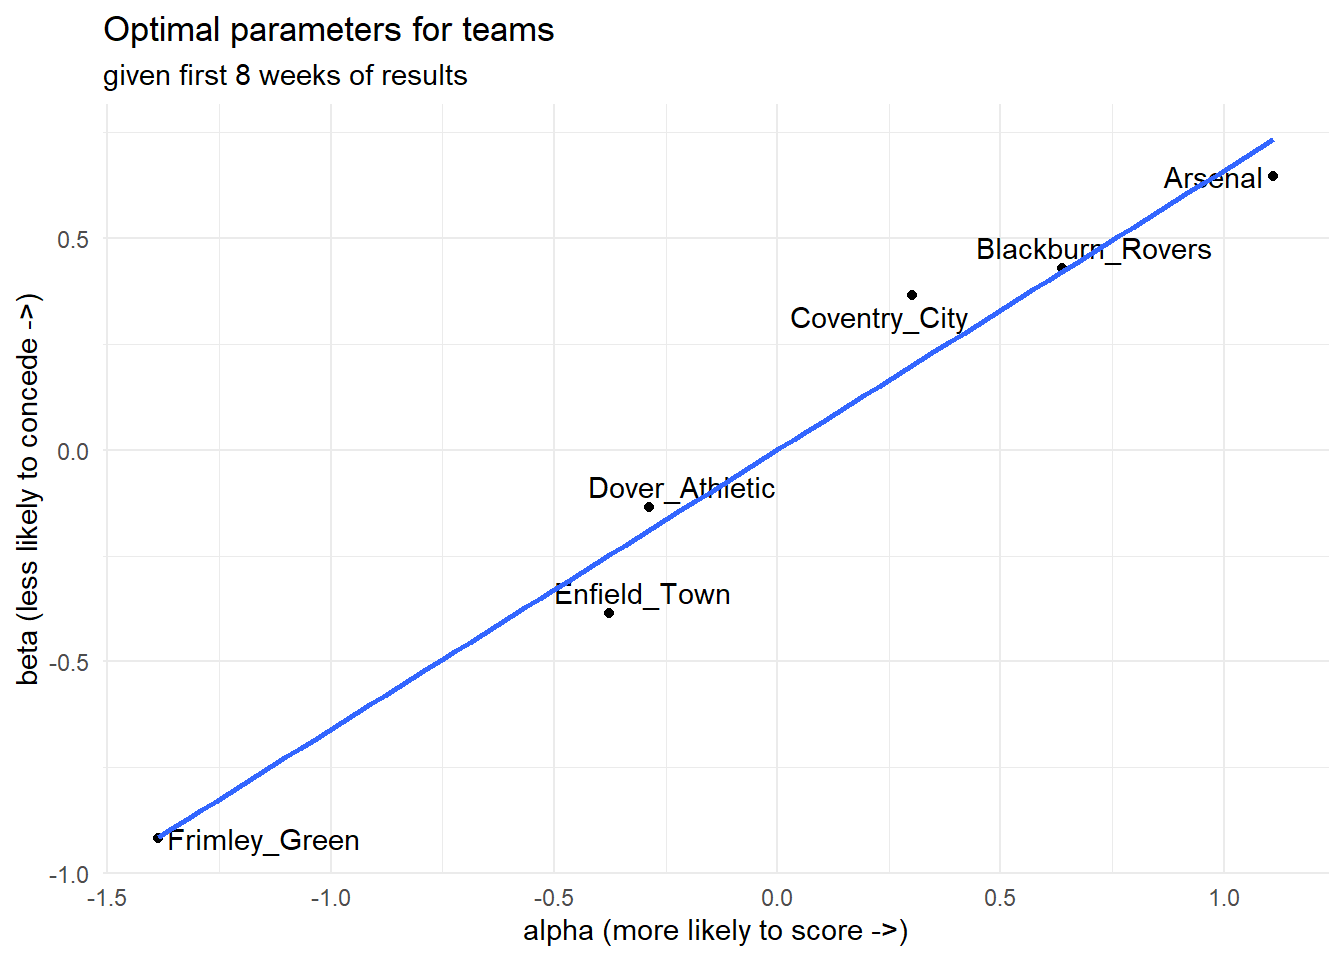
\includegraphics{dixon_coles_1_files/figure-latex/plot_parameters-1.pdf}


\end{document}
